\chapter{CodFS Design}
\label{chap:codfs}

\section{Parity Updates}
\label{sec:parity}

%In a traditional file system, handling update writes is a trivial problem. All
%we have to do is to overwrite the existing data with a newer version. However,
%things become more complicated in an erasure coding file system. In addition to
%the data, we also need to update the parity accordingly. Otherwise, data
Data updates in erasure-coded clustered storage systems introduce performance
overhead, since they also need to update parity chunks for consistency.  We
consider a deployment environment where network transfer and disk I/O are
performance bottlenecks.  Our goal is to design a parity update scheme that
effectively mitigates both network transfer overhead and number of disk seeks.

%Different methods have been proposed to improve the performance of parity
%updates. However, most of them address the problem from a single-host (e.g.,
%RAID) perspective, while in a distributed setting we also need to take the
%network transfer overhead into design consideration.  

We re-examine existing parity update schemes
%and evaluate the feasibility of
%adopting these approaches in erasure-coded clustered storage systems.  We
%first study 
that fall into two classes: the RAID-based approaches and the delta-based
approaches. 
%We discuss their strengths and drawbacks. 
We then propose a novel parity update approach that assigns a reserved space
for keeping parity updates. 
%and how we control the size of such space.

\subsection{Existing Approaches}

\subsubsection{RAID-based Approaches}

We describe three classical approaches of parity updates that are typically
found in RAID systems \cite{chen95,thomasian05}. 

%\red{Should we use ``stripe,block'' in pair or ``segment, chunk'' in pair ?}

\paragraph{Full-segment writes.} A full-segment write (or full-stripe write)
updates all data and parity chunks in a segment. 
It is used in a large sequential
write where the write size is a multiple of segment size.  To make a
full-segment write work for small updates, one way is to pack several updates
into a large piece until a full segment can be written in a single operation 
\cite{menon95}. Full-segment writes do not need to read the old data or parity
chunks, and hence achieve the best update performance.

%For instance, in log-structured arrays (LSAs), a cache is used to accumulate
%modified chunks until a full segment can be written in a single operation

\paragraph{Reconstruct writes.} A reconstruct write first reads all the chunks
from the segment that are not involved in the update.  Then it computes the new parity chunks
using the read chunks and the new chunks to be written, and writes all data
and parity chunks. 
%other than the ones currently writing to are read. We then compute a new parity
%based on these chunks. After that, we simply replace the old parity with the
%new one.

\paragraph{Read-modify writes.} A read-modify write leverages the linearity of
erasure coding for parity updates (see \S\ref{sec:ec_background}).  It first
reads the old data chunk to be updated and all the old parity chunks in the
segment.  It then computes the change between the old and new data chunks, and
applies the change to each of the parity chunks. 
%Next, we compute the new parity chunk by XOR the parity update with the old
%parity chunk. 
Finally, it writes the new data chunk and all new parity chunks to their
respective locations. 
%Therefore, updating a single chunk with single parity by read-modify write
%requires 4 I/O operations, reading and writing both data chunk and parity
%chunk.

\paragraph{Discussion.}  Full-segment writes can be implemented through a
log-based design to support small updates, but logging has two limitations.
First, we need an efficient garbage collection mechanism to reclaim space by
removing stale chunks, and this often hinders update performance
\cite{seltzer95}. Second, logging introduces additional disk seeks to retrieve
the updates, which often degrades sequential read and recovery performance
\cite{matthews97}. 
On the other hand, both reconstruct writes and read-modify writes 
%mitigate the fragmentation of log-structured file systems through in-place
%updates.  However, they 
are traditionally designed for a single host deployment. Although some recent
studies implement read-modify writes in a distributed setting
\cite{frolund04,zhang12}, both approaches
introduce significant network traffic since each update must transfer data or
parity chunks between nodes for parity updates. 

%Using reconstruct write approach in a distributed file system would introduce an excessive amount of inter-node network traffic since for each update, we need to transfer data chunks between nodes in order to update the parity. The read-modify write approach also introduces unnecessary network traffic, especially when the update size is far smaller than the chunk size. 

%Compared with the classical approaches, delta-based techniques are more
%suited in a distributed environment.

\begin{figure*}[!t]
    \centering
    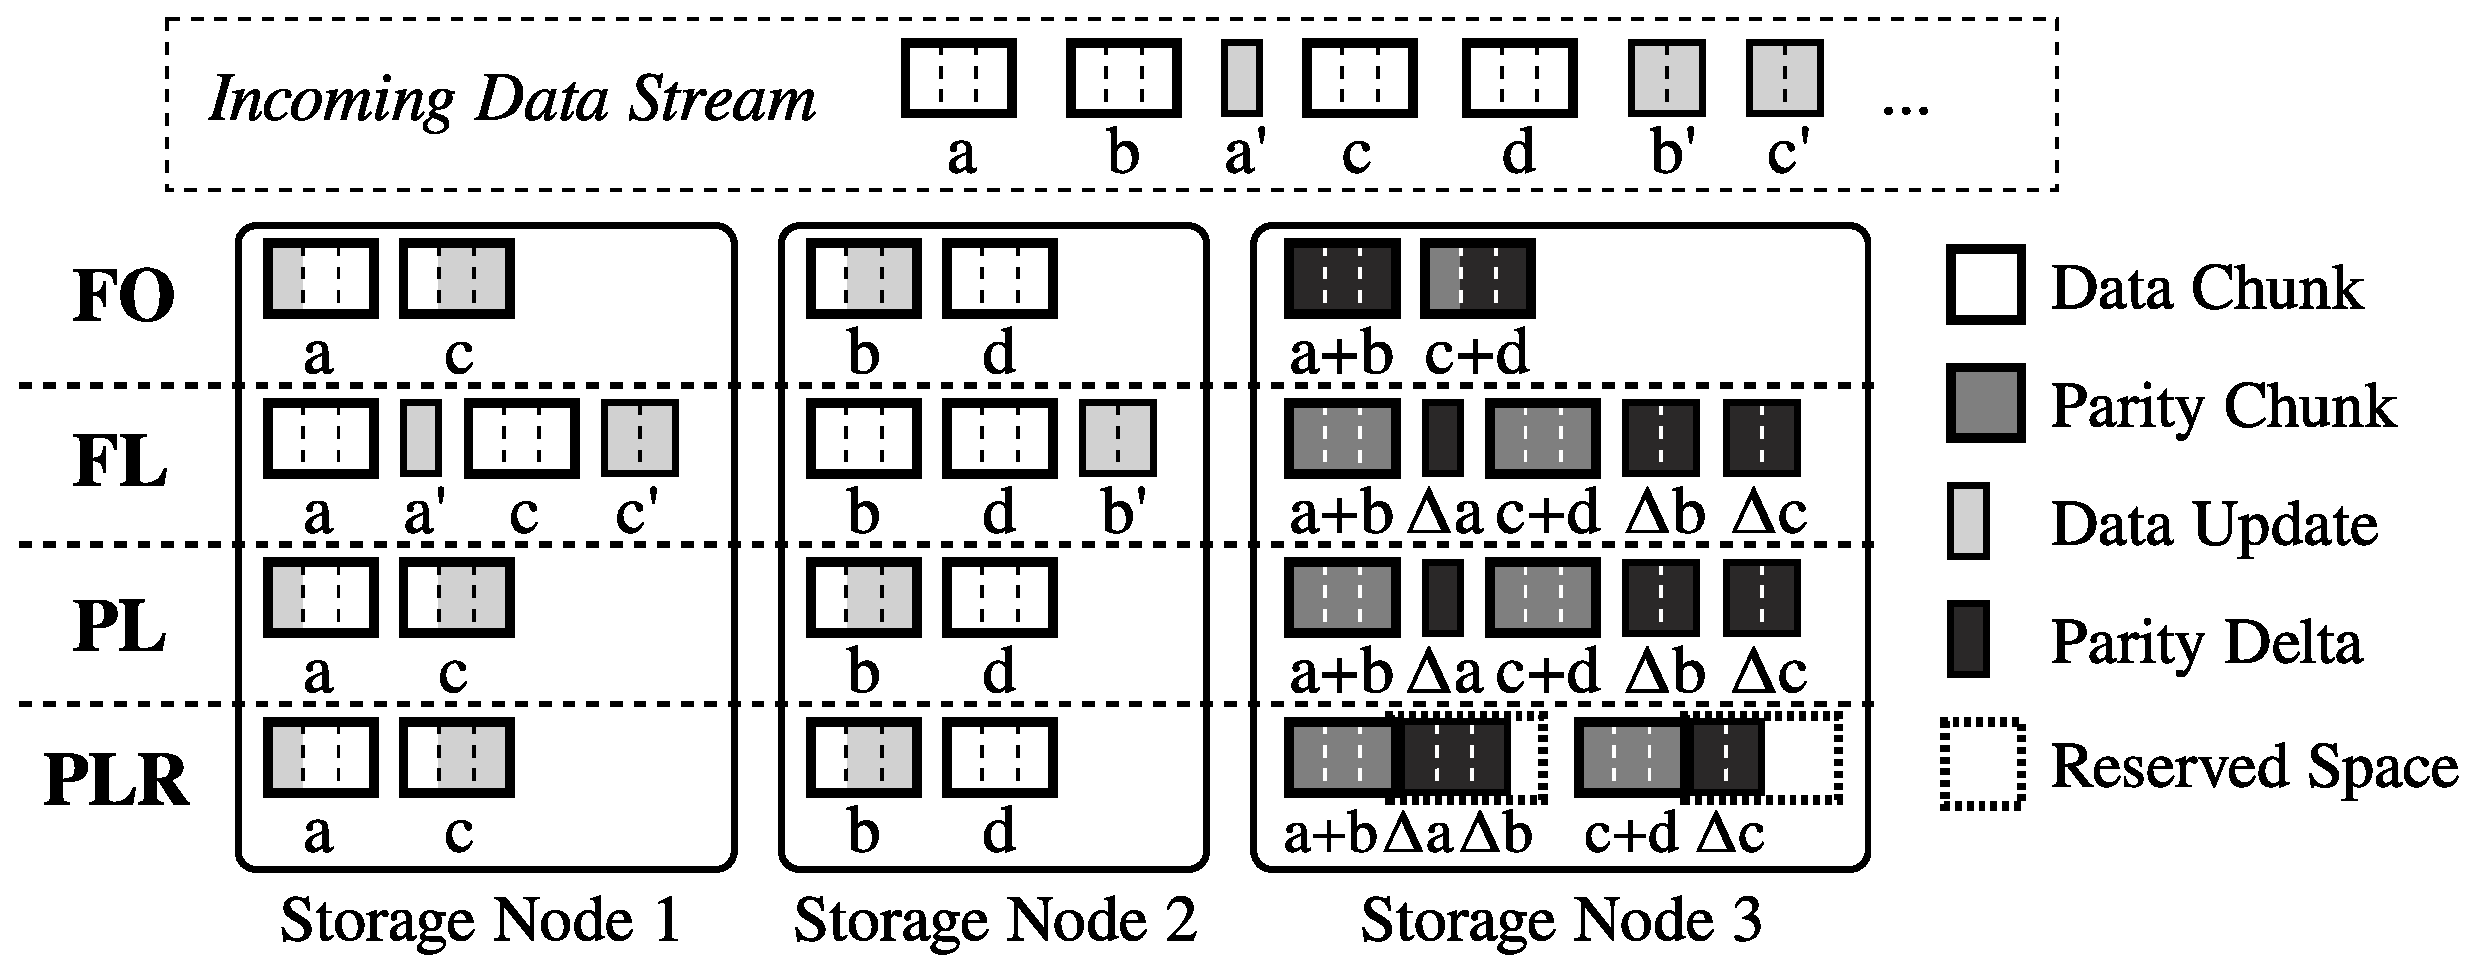
\includegraphics[width=4.8in]{figs/schemes_chunkflow}
%    \hspace{-3pt}
    \vspace{-3pt}
    \caption{Illustration on different parity update schemes.}
    \label{fig:schemes_chunkflow}
\end{figure*}

\subsubsection{Delta-based Approaches}
\label{sec:delta_based}

Another class of parity updates, called the {\em delta-based approaches}, 
eliminates redundant network traffic by only transferring a {\em parity delta}
which is of the same size as the modified data range~\cite{cao94,storer08}.  A
delta-based approach
leverages the linearity of erasure coding described in
\S\ref{sec:ec_background}. It first reads the range of the data chunk to be
modified and computes the delta, which is the change between old and new data at the modified 
range of the data chunk, for each parity chunk. It then sends the
modified data range and the parity deltas computed to the data node and all
other parity nodes for updates, respectively. 
%both the data and parity chunks are no longer required to be fully read
%for computing and applying delta when the update is smaller than chunk size. 
Instead of transferring the entire data and parity chunks as in
read-modify writes, transferring the modified data range and parity deltas
reduces the
network traffic and is suitable for clustered storage.  In the following, we
describe some delta-based approaches proposed in the literature. 

%Meanwhile, the network traffic for transferring delta 
%between the data node and parity node can be reduce.
%updating existing stripes in a erasure-coded and 
%distributed storage setting. 

%According to the trace analysis, the update size is often much smaller than
%chunk size.  Hence, for such small updates, using traditional
%read-modify-write scheme is still not optimal.  As traditional read-modify-write
%scheme computes parity updates using the unit of chunk size, this scheme
%still generates extra traffic caused by those non-modified content within a
%chunk. Here, we examine four different approaches for saving the data update
%or parity deltas on disk.

\paragraph{Full-overwrite (\FO).} Full-overwrite
\cite{aguilera05} applies in-place updates
to both data and parity chunks. It merges the old data and parity chunks
directly at specific offsets with the modified data range and parity deltas,
respectively. Note that merging each parity delta requires an additional disk read of
old parity chunk at the specific offset to compute the new parity content to be
written.
%The baseline approach is the fully-overwrite approach, which requires the
%same number of disk I/O as the read-modify-write The data update overwrites
%the original data chunk 
%after the corresponding parity delta is computed.
%The parity delta is then sent to the parity location and merged into the
%original parity chunk by performing XOR between the delta and the old parity.
%Two read operations and two write operations are required in this approach. 

\paragraph{Full-logging (\FL).} Full-logging saves the disk read overhead of
parity chunks by appending all data and parity updates. 
That is, after the modified data
range and parity deltas are respectively sent to the corresponding data and
parity nodes, the storage nodes create logs to store the updates.  The logs
will be merged with the original chunks when the chunks are read subsequently.
\FL is used in enterprise clustered storage systems such as 
GFS \cite{ghemawat03} and Azure \cite{calder11}. 

\paragraph{Parity-logging (\PL).} Parity-logging \cite{stodolsky93,jin11}
can be regarded as a hybrid of \FO and \FL.  It saves the disk read overhead of
parity chunks and additionally avoids merging overhead on data chunks introduced in \FL.
Since data chunks are more likely to be read than parity chunks,
merging logs in data chunks can significantly degrade read 
performance. Hence, in \PL, the original data chunk is overwritten in-place with the
modified data range, while the parity deltas are logged at the parity nodes.
%Hence, there is also no disk read for the parity chunks on the update path.
%The parity chunks will be merged with the parity deltas when they are accessed
%(e.g., during recovery). 

\paragraph{Discussion.} 
Although the delta-based approaches reduce network traffic,
they are not explicitly designed to reduce disk I/O. Both \FL
and \PL introduce disk fragmentation and require efficient garbage
collection. The fragmentations often hamper further 
accesses of those chunks with logs. Meanwhile, \FO introduces additional disk reads
for the old parity chunks on the update path, compared with \FL and \PL.
Hence, to take a step further, we want to address the question: 
\textit{Can we reduce the disk I/O on both the update path and further
accesses?}  

\subsection{Our Approach}

We propose a new delta-based approach called {\bf parity-logging with reserved
space (\PLR)}, which further mitigates fragmentation and reduces the disk seek
overhead of \PL in storing parity deltas.  The main idea is that the storage
nodes reserve additional storage space next to each parity chunk for keeping 
parity deltas.  This ensures that each parity chunk and its parity deltas
can be sequentially retrieved. While the idea is simple, the challenging
issues are to determine (1) the appropriate amount of reserved space to be
allocated when a parity chunk is first stored and (2) the appropriate time
when unused reserved space can be reclaimed to reduce the storage overhead. 

%Subsequent deltas are logged in the reserved space. Once the reserved space
%for a parity chunk is full, the storage node takes a merge operation,
%applying the logs in the reserved space to the parity chunk and clears
%the reserved space for subsequent deltas.  

\subsubsection{An Illustrative Example} 

Figure~\ref{fig:schemes_chunkflow} illustrates the differences of the
delta-based approaches in \S\ref{sec:delta_based} and \PLR, using a
(3,2)-code as an example.  The incoming data stream describes the sequence of
operations: (1) write the first segment with data chunks \texttt{a} and
\texttt{b}, (2) update part of \texttt{a} with \texttt{a'}, (3) write a new
segment with data chunks \texttt{c} and \texttt{d}, and finally (4) update parts
of \texttt{b} and \texttt{c} with \texttt{b'} and \texttt{c'}, respectively.  We
see that \FO performs overwrites for both data updates and parity deltas; \FL
appends both data updates and parity deltas according to the incoming order; \PL
performs overwrites for data updates and appends parity deltas; and \PLR appends
parity deltas in reserved space. 

Consider now that we read the up-to-date chunk \texttt{b}.  \FL incurs a disk
seek to the update \texttt{b'} when rebuilding chunk \texttt{b}, as 
\texttt{b} and \texttt{b'} are in discontinuous physical locations on
disk.  Similarly, \PL also incurs a disk seek to the parity delta
\texttt{$\Delta$b} when reconstructing the parity chunk \texttt{a+b}. On the
other hand,  $\PLR$ incurs no disk seek when reading the parity chunk 
\texttt{a+b} since its parity deltas \texttt{$\Delta$a} and \texttt{$\Delta$b} are all placed
in the contiguous reserved space following the parity chunk \texttt{a+b}. 

\section{Determination of Reserved Space Size}
\label{sec:reserve_strategies}

Finding the appropriate reserved space size is challenging.  If the space is
too large, then it wastes storage space.   On the other hand, if the space is
too small, then it cannot keep all parity deltas.  

%Thus, before storing the
%coming delta, when the reserved space is full, a \textit{merge} operation is 
%first performed to apply the deltas in the reserved space to the parity
%chunk. In the worst case, the update performance can downgrade to the \FO
%approach if the parity chunk needs to be merged every time.

%The \PLR approach avoid the parity fragmentation by preallocating a reserved
%space. However, it also introduces merging overhead once the reserved space
%is full. Hence, we intend to minimize the number of merge operations since
%latency increases when updates are stalled during a merge.  Although using a
%larger reserved space can effectively prevents merging, it introduces
%unnecessary storage space overhead. 

%\red{the alternatives' name may be discussed}

A baseline approach is to use a fixed reserved space size for each parity
chunk, where the size is assumed to be large enough to fit all parity deltas.  
Note that this baseline approach can introduce
significant storage overhead, since different segments may have different
update patterns.  For example, from the Harvard NFS traces shown in
Table~\ref{table:harvard}, although $91.56\%$ of write requests are updates,
only around $12\%$ of files are actually involved.  This uneven distribution
implies that fixing a large, constant size of reserved space can imply
unnecessary space wastage. 

For some workloads, the baseline approach may reserve insufficient space to
hold all deltas for a parity chunk. There are two alternatives to handle extra
deltas, either logging them elsewhere like \PL, or \textit{merging} existing
deltas with the parity chunk to reclaim the reserved space.  We adopt the
merge alternative since it preserves the property of no fragmentation in
\PLR.

To this end, we propose a workload-aware reserved space management scheme that
dynamically adjusts and predicts the reserved space size. The scheme has
three main parts: 
(1) predicting the reserved space size of each parity chunk 
using the measured workload pattern for the next time interval, 
(2) shrinking the reserved space and releasing unused reserved space back to 
the system, and
(3) merging parity deltas in the reserved space to each parity chunk.
To avoid introducing small unusable holes of reclaimed space after shrinking,
we require that both the reserved space size and the shrinking size be of
multiples of the chunk size.  This ensures that an entire data or parity chunk
can be stored in the reclaimed space. 

\begin{algorithm}[t]
\DontPrintSemicolon
$\emph{reserved} \gets $\verb|DEFAULT_SIZE|\;
\While{$\rm{true}$}{
  \KwSty{sleep}$(\emph{period})$\;
  \ForEach{chunk \textbf{\emph{in}} parityChunkSet}{
  $\emph{utility} \gets $ \FuncSty{getUtility}$(\emph{chunk})$ \;
  $\emph{size} \gets $ \FuncSty{computeShrinkSize}$(\emph{utility})$ \;
    %$size \gets $ \KwSty{roundToChunk}$(size)$ \;
    \FuncSty{doShrink}$(\emph{size}, \emph{chunk})$  \label{line:deallocate} \;
    \FuncSty{doMerge}$(\emph{chunk})$ \;
  }
%  \del{$\emph{reserved} \gets$ \FuncSty{predict}$(\emph{parityChunkSet})$}% \;}
}
\caption{Workload-aware Reserved Space Management}
\label{alg:deallocate}
\end{algorithm}

Algorithm~\ref{alg:deallocate} describes the basic framework of our
workload-aware reserved space management.  Initially, we set a default
reserved space size that
is sufficiently large to hold all parity deltas.  Shrinking and
prediction are then executed periodically on each storage node.  Let
$\mathcal{S}$ be the set of parity chunks in a node. For every time interval
$t$ and each parity chunk $p\in \mathcal{S}$, let $r_t(p)$ be the reserved
space size and $u_t(p)$ be the reserved space utility.   Intuitively, $u_t(p)$
represents the fraction of reserved space being used.  We measure $u_t(p)$ at
the end of each time interval $t$ using exponential weighted moving average
in \texttt{getUtility}:
%
\begin{equation*} \label{eq:utility_now}
    u_t(p)  = \alpha \frac{\emph{use}(p)}{r_{t}(p)} + (1-\alpha)u_{t-1}(p),
\end{equation*} 
%
where $\emph{use}(p)$ returns the reserved space size being used during the
time interval, $r_{t}(p)$ is the current reserved space size for chunk
$p$, and $\alpha$ is the smoothing factor.  
%We set $\alpha =0.05$ by default as the smoothing factor.  
According to the utility, we decide the unnecessary space size $c(p)$ that can
be reclaimed for the parity chunk $p$ in \texttt{computeShrinkSize}.  Here, we
aggressively shrink all unused space $c(p)$ and round it down to be a multiple
of the chunk size:
%
\begin{equation*} \label{eq:shrink_size}
%    c_p = c_p^{*} - (c_p^{*}\bmod ChunkSize)
	c(p) = \left\lfloor\frac{(1-u_{t}(p))r_{t}(p)}{ChunkSize}\right\rfloor
	\times ChunkSize.
\end{equation*} 

The \texttt{doShrink} function attempts to shrink the size $c(p)$ from the
current reserved space $r_{t}(p)$. Thus, the reserved space $r_{t+1}(p)$ 
for $p$ at time interval $t+1$ is: 
$$
r_{t+1}(p) = r_{t}(p) - c(p).
$$
%
If a chunk has no more reserved space after shrinking (i.e., $r_{t+1}(p)
= 0$), any subsequent update requests to this chunk are applied in-place as
in \FO.

Finally, the \texttt{doMerge} function merges the deltas in the reserved space
to
the parity chunk $p$ after shrinking and resets $\emph{use(p)}$ to zero. Hence
we free the parity chunk from carrying any deltas to the next time interval,
which could further reduce the reserved space size.  The merge operations
performed here are off the update path and have limited impact on the overall
system performance. 

%\del{Finally, we predict the reserved space size $R_{t+1}$ for the new parity
%chunks in the next time interval $t$ based on the average reserved space size
%of all existing parity chunks.  We also apply exponential weighted moving
%average on the prediction:}
%\begin{equation*} \label{eq:predict}
%    \del{
%R_{t+1} = \left\lfloor\frac{\beta \frac{\sum_{p\in \mathcal{S}}
%	r_{t+1}(p)}{|\mathcal{S}|} + (1-\beta) R_{t}}{ChunkSize}\right\rfloor
%	\times ChunkSize,
%%    P_{t+1} = P_{t+1}^{*} - (P_{t+1}^{*}\bmod ChunkSize)
%}
%\end{equation*} 
%\del{where $R_{t}$ is the predicted reserve space size for current time interval
%$t$ and we set $\beta = 0.05$ for the smoothing factor by default. We also
%adjust the prediction size to be a multiple of the chunk size.}

%heuristic we present for measurement and prediction in the framework is 
The above workload-aware design of reserved space management is simple and can
be replaced by a more advanced design.  Nevertheless, we find that this simple
heuristic works well enough under real-world workloads (see
\S\ref{eval:reserve_evaluation}). 

%\paragraph{Shrink with Merge.}
%We further propose the third strategy. 
%While the basic flow remains the same, 
%we perform a merge after shrinking the reserved space for each parity chunk, i.e. after
%line~\ref{line:deallocate} in Algorithm~\ref{alg:deallocate}. Hence we free the parity
%chunks from carrying any deltas to the next period, which 
%could further reduce the reserved space size.
%Also, performing merge operation off the update path have less impact on the
%entire system performance. Thus,
%we expected it to be more effective than the previous shrinking approach.

%Reserving space for parity chunk can be implemented by calling \texttt{fallocate}, which
%also supports shrinking the reserved space by specifying the
%\texttt{FALLOC\textunderscore FL\textunderscore PUNCH\textunderscore HOLE} flag.
%The overhead of calling \texttt{fallocate} for reserving or shrinking is
%negligible. Therefore, we expect the shrinking job does not hurt the system
%performance and we will evaluate the three strategies in
%\S\ref{sec:reserve_evaluation}. 

